

\section{Research}
This research project is a continuation of a previous research project done by Heiko van der Heijden. His results show that of the two algorithms tested, Re-initialization and Blacklist, that the Blacklist algorithm has fewer Time Frames lost. (van der Heijden, 2018, p. 43)\\
Even though the same ratio of FLPs to EPNs that is situated at CERN was used (1/6), there were fewer computers used than at CERN. Because of this it is not sure whether or not the Information Node is able to handle 1700+ computers as compared to the 15 computers used in the experiment. This research is focused on the capability of the Information Node to monitor a higher number of FLPs and EPNs and what the effects are on the results compared to the previous experiment.\\

\section{Research Model}
Contrary to the previous research, which used a cluster of computers situated at Nikhef Amsterdam, this research will be conducted using a cluster of Raspberry Pi's. This decision has been made because of an unfortunate failure of communication from Nikhef about the availability of the cluster for this research period. The first step is to recreate the previous experiment which was focused around the various ticktimes of Zookeeper.
\newpage

~\\\textbf{The main purpose of this research is to both validate the results from the previous experiment, but also to validate the new Raspberry Pi cluster to confirm that this is a valid way to conduct this experiment. After recreating the first experiment, the same experiment will be conducted with a higher numbers of computers to see if this has an effect on the Information Node. Finally an experiment will be conducted to see whether the layout of the system architecture is of influence for the TF loss.} \\~\\
An overview can be seen in figure ~\ref{fig:ResearchModel}

\begin{figure}[htb]
	\centering
	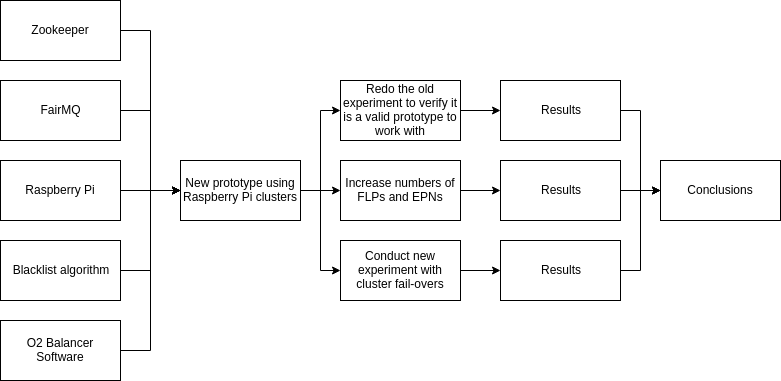
\includegraphics[width=\textwidth,height=\textheight,keepaspectratio]{./graphics/ResearchModel.png}
	\caption{Research model}
	\label{fig:ResearchModel}
\end{figure}

~\\ All technical documentation of what everything is will be explained in the next section including the definition of the experiments.
The next chapter will explore more in depth of the prototype made for the experiment and it's difficulties that came with it. The following chapter looks at the results from the  executed experiments. After this follows an analysis of the results of the experiment. Finally a conclusion and recommendations.